\documentclass[12pt,letterpaper]{article}
\usepackage{graphicx,textcomp}
\usepackage{natbib}
\usepackage{setspace}
\usepackage{fullpage}
\usepackage{color}
\usepackage[reqno]{amsmath}
\usepackage{amsthm}
\usepackage{fancyvrb}
\usepackage{amssymb,enumerate}
\usepackage[all]{xy}
\usepackage{endnotes}
\usepackage{lscape}
\newtheorem{com}{Comment}
\usepackage{float}
\usepackage{hyperref}
\newtheorem{lem} {Lemma}
\newtheorem{prop}{Proposition}
\newtheorem{thm}{Theorem}
\newtheorem{defn}{Definition}
\newtheorem{cor}{Corollary}
\newtheorem{obs}{Observation}
\usepackage[compact]{titlesec}
\usepackage{dcolumn}
\usepackage{tikz}
\usetikzlibrary{arrows}
\usepackage{multirow}
\usepackage{xcolor}
\newcolumntype{.}{D{.}{.}{-1}}
\newcolumntype{d}[1]{D{.}{.}{#1}}
\definecolor{light-gray}{gray}{0.65}
\usepackage{url}
\usepackage{listings}
\usepackage{color}

\definecolor{codegreen}{rgb}{0,0.6,0}
\definecolor{codegray}{rgb}{0.5,0.5,0.5}
\definecolor{codepurple}{rgb}{0.58,0,0.82}
\definecolor{backcolour}{rgb}{0.95,0.95,0.92}

\lstdefinestyle{mystyle}{
	backgroundcolor=\color{backcolour},   
	commentstyle=\color{codegreen},
	keywordstyle=\color{magenta},
	numberstyle=\tiny\color{codegray},
	stringstyle=\color{codepurple},
	basicstyle=\footnotesize,
	breakatwhitespace=false,         
	breaklines=true,                 
	captionpos=b,                    
	keepspaces=true,                 
	numbers=left,                    
	numbersep=5pt,                  
	showspaces=false,                
	showstringspaces=false,
	showtabs=false,                  
	tabsize=2
}
\lstset{style=mystyle}
\newcommand{\Sref}[1]{Section~\ref{#1}}
\newtheorem{hyp}{Hypothesis}

\title{Problem Set 4}
\date{Due: April 16, 2023}
\author{Applied Stats II}


\begin{document}
	\maketitle
	\vspace{.25cm}
\section*{Question 1}
\vspace{.25cm}
\noindent We're interested in modeling the historical causes of infant mortality. We have data from 5641 first-born in seven Swedish parishes 1820-1895. Using the "infants" dataset in the \texttt{eha} library, fit a Cox Proportional Hazard model using mother's age and infant's gender as covariates. Present and interpret the output.


\begin{lstlisting}[language=R]

# Load data
data(child)
head(child)

# Build a survival object out of the `child` data.frame
child_surv <- with(child, Surv(enter, exit, event))

# Run a Cox Proportional Hazard regression
cox <- coxph(child_surv ~ m.age + sex, data = child)
summary(cox)
drop1(cox, test = "Chisq")
stargazer(cox, type = "text")
	
\end{lstlisting}

\noindent 
We can plot this survival function using a Kaplan Meyer plot: 

\begin{lstlisting}[language=R]
# Plot 
km <- survfit(child_surv ~ 1, data = child)
summary(km, times = seq(0, 15, 1))
plot(km, main = "Kaplan-Meier Plot", xlab = "Years", ylim = c(0.7, 1))
\end{lstlisting}

\begin{figure}
	\centering
	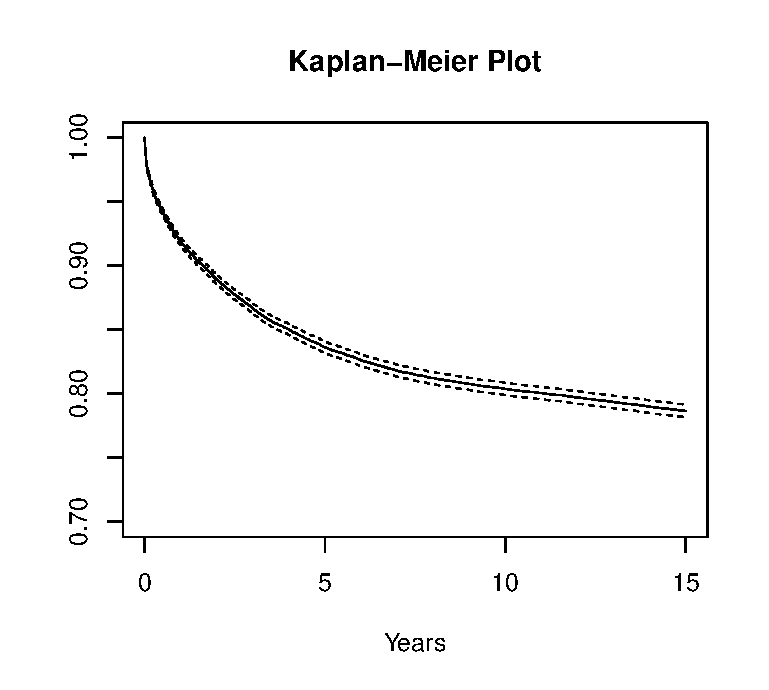
\includegraphics[width=4.0in]{KaplanMeier_ChildSurv.pdf}
	\caption{Child Survival Kaplan Meier plot}
	\label{Fig1}
\end{figure}

\begin{lstlisting}[language=R]
# Run a Cox Proportional Hazard regression
cox <- coxph(child_surv ~ m.age + sex, data = child)
summary(cox)
drop1(cox, test = "Chisq")
stargazer(cox, type = "text")

\end{lstlisting}

\noindent Please view output on next page: \\

% Table created by stargazer v.5.2.3 by Marek Hlavac, Social Policy Institute. E-mail: marek.hlavac at gmail.com
% Date and time: Sun, Apr 16, 2023 - 18:27:00
\begin{table}[!htbp] \centering 
	\caption{} 
	\label{} 
	\begin{tabular}{@{\extracolsep{5pt}}lc} 
		\\[-1.8ex]\hline 
		\hline \\[-1.8ex] 
		& \multicolumn{1}{c}{\textit{Dependent variable:}} \\ 
		\cline{2-2} 
		\\[-1.8ex] & child\_surv \\ 
		\hline \\[-1.8ex] 
		m.age & 0.008$^{***}$ \\ 
		& (0.002) \\ 
		& \\ 
		sexfemale & $-$0.082$^{***}$ \\ 
		& (0.027) \\ 
		& \\ 
		\hline \\[-1.8ex] 
		Observations & 26,574 \\ 
		R$^{2}$ & 0.001 \\ 
		Max. Possible R$^{2}$ & 0.986 \\ 
		Log Likelihood & $-$56,503.480 \\ 
		Wald Test & 22.520$^{***}$ (df = 2) \\ 
		LR Test & 22.518$^{***}$ (df = 2) \\ 
		Score (Logrank) Test & 22.530$^{***}$ (df = 2) \\ 
		\hline 
		\hline \\[-1.8ex] 
		\textit{Note:}  & \multicolumn{1}{r}{$^{*}$p$<$0.1; $^{**}$p$<$0.05; $^{***}$p$<$0.01} \\ 
	\end{tabular} 
\end{table} 

\vspace{.10cm}


\textbf{Analysis:} 
\noindent The results show that both mother's age and infant's gender are statistically significant predictors of child mortality, with p-values less than 0.01.

For mother's age, the coefficient estimate of 0.008 indicates that for each one-year increase in mother's age, the hazard of child mortality increases by a factor of 1.008 (exp(0.008)).

For infant's gender, the coefficient estimate of -0.082 indicates that the hazard of mortality is lower for female infants than for male infants by a factor of 0.921 (exp(-0.082)). 

The drop1() function allows us to asses the  model quality by removing each predictor one at a time from the model and comparing the fit of the reduced model to the original model using an LRT.
\\

\begin{Verbatim}
	> drop1(cox, test = "Chisq")
	Single term deletions
	
	Model:
	child_surv ~ m.age + sex
	Df    AIC     LRT  Pr(>Chi)    
	<none>    113011                      
	m.age   1 113022 12.7946 0.0003476 ***
	sex     1 113018  9.4646 0.0020947 ** 
	---
	Signif. codes:  0 ‘***’ 0.001 ‘**’ 0.01 ‘*’ 0.05 ‘.’ 0.1 ‘ ’ 1
\end{Verbatim}

\noindent Here we can see that that removing either mother's age or infant's gender from the model leads to a significant deterioration in the model fit based on the likelihood ratio test. This indicates that both predictors are important in predicting child survival. 

















\end{document}


